\section{Scheduling \weekDoran{2}}
	\begin{tabular}{p{0.475\textwidth}p{0.475\textwidth}}
		\begin{compactitem}
		  \item The scheduling diagram indicates how much time is necessary for each of the tasks, how much time is left until the cycle time is is reached and which system architecture element is affected by which task.
		  \item If the same task is affected by multiple elements, that is indicated by showing that this runs at the same time, not after one another. Otherwise it should be split into multiple tasks.
		  \item The tasks in the scheduling diagram are the same tasks as drawn in the left part of the binding diagram.
		\end{compactitem}
		& \vspace{0pt}
		
		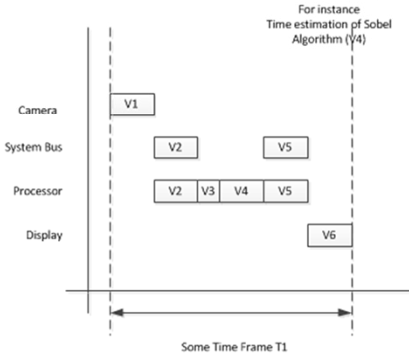
\includegraphics[width=0.35\textwidth]{./pictures/scheduling.png}\\
	\end{tabular}	
	
	\subsection{Scheduling Time Measurements}
	\begin{table}[H]\centering
		\begin{tabular}{|>{\bfseries}p{0.25\linewidth}|p{0.7\linewidth}|}
			\hline
				Slack
					& The time that is left until the maximum cycle time is reached.\\
			\hline
				Idle time
					& The time that the CPU is waiting for other elements to finish their tasks.\\
			\hline
				Maximum task scaling factor
					& The factor, by which the time spent in the CPU's tasks can be multiplied so that the idle time is exactly the time that the other elements require while the CPU is idle: \newline 
					{$T_{IdleNew} = T_{CycleMax} - x \cdot T_{CPU} = T_{OtherElem}$} $\rightarrow$
					{$x = \frac{T_{CycleMax} - T_{OtherElem}}{T_{CPU}}$} \newline
					This implies that the complete cycle time is being used!\\
			\hline
		\end{tabular}
	\end{table}
	
	\subsection{List Scheduling}
		The algorithm of list scheduling goes as follows:
		
		\begin{compactenum}
			\item Order tasks with decreasing (static) priority.
			\item Repeat until a valid schedule is obtained:
			\begin{compactenum}
			  \item Select the task with the highest priority.
			  \item Select a resource to accommodate this task.
			  \item If no resource can be found, select next task in the list.
			\end{compactenum}
		\end{compactenum}
		
		\begin{table}[H]\centering
			\begin{tabular}{p{0.425\linewidth}p{0.425\linewidth}}
				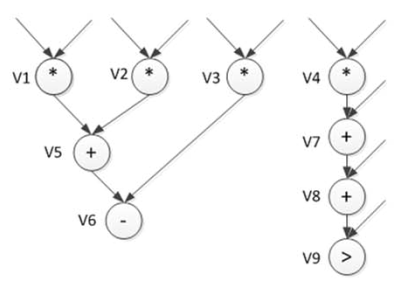
\includegraphics[scale=0.8]{./pictures/listSchedDiag.png}
				& 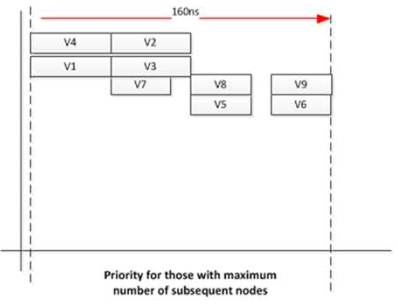
\includegraphics[scale=0.8]{./pictures/listSched.png}\\
			\end{tabular}
		\end{table}

	\subsection{First Come First Served Scheduling}
		Is a non-preemptive scheduling technique. Starvation is not an issue, since there is no priority assigned to tasks. However, fairness is an issue because long tasks dominate.
		\begin{figure}[H]\centering
			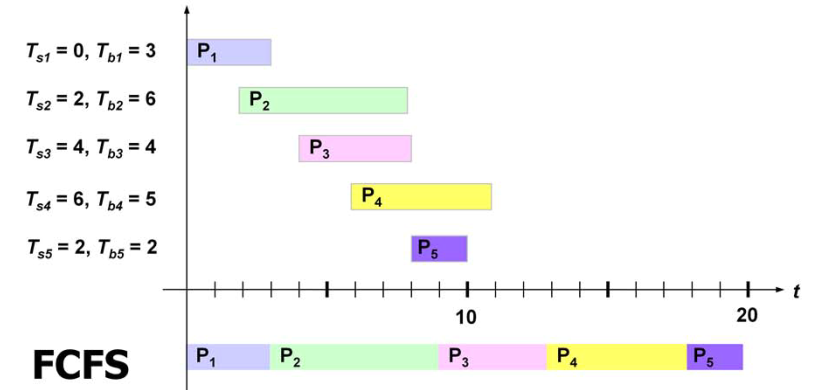
\includegraphics[scale=0.5]{./pictures/firstComeFirstServe.png}
		\end{figure}
			
	\subsection{Round Robin Scheduling}
		Round Robin scheduling is in essence a FIFO with preemption. Represents Time Division multiplexing in HW terms.
		
		The execution time is divided up into time slices, each task gets to run for a time slice, after which the next task is allowed to do the same. This algorithm is starvation-free.

		Conditions for operation:
		\begin{compactitem}
		  \item Tasks need to be preemptive
		\end{compactitem}
		
		\begin{figure}[H]\centering
			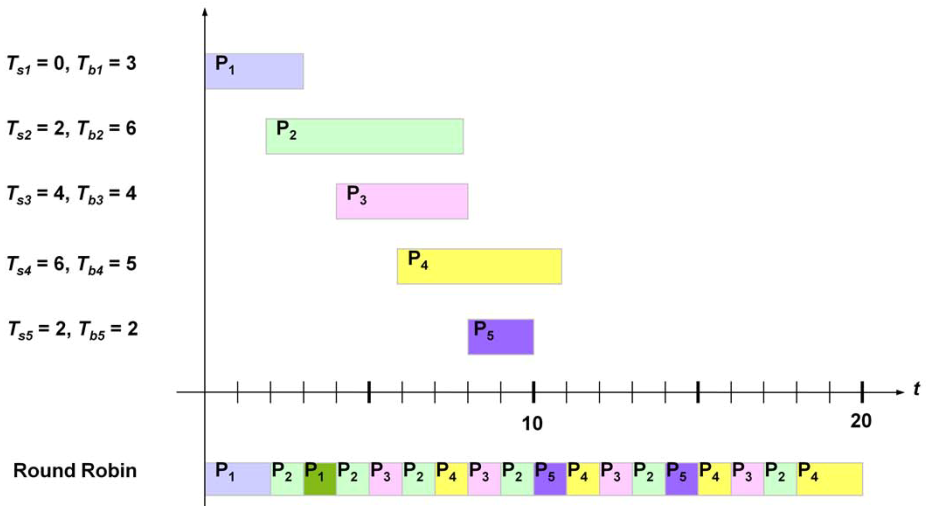
\includegraphics[scale=0.5]{./pictures/roundRobin.png}
		\end{figure}
		
	\subsection{Rate Monotonic Scheduling}
		Rate monotonic scheduling assigns a higher priority the highest repetition rate of a task, i.e. a task that has the shortest period has the highest priority. It is a preemptive scheduling technique.
		
		Conditions for operation:
		\begin{compactitem}
		  \item Tasks need to be preemptive
		  \item Tasks need deterministic deadlines
		\end{compactitem}
		
		A sufficient (but not necessary) condition for a set of tasks with unique periods to be schedulable is:		
		\begin{equation*}
			\begin{aligned}
				U &= \sum_{i=1}^{n} \frac{C_i}{T_i} \leq n(\sqrt[n]{2}-1)\\
				U &= \text{CPU utilisation}\\
				n &= \text{Number of tasks}\\
				C_{i} &= \text{Computation time} \\
				T_{i} &= \text{Release period (one period before the deadline)}\\
			\end{aligned}
		\end{equation*}
		
		Since this condition is not necessary, it means that a well designed system could still schedule these tasks with a higher CPU utilisation.
		
		\begin{compactitem}
		  \item At $t = 0$ all periods start running.
		  \item A task is only interrupted if a task with higher priority is in the queue.
		  \item A task leaves the queue when it is executed to completion or when its period starts again.
		\end{compactitem}

		\begin{table}[H]\centering
			\begin{tabular}{p{0.7\linewidth}p{0.25\linewidth}}
				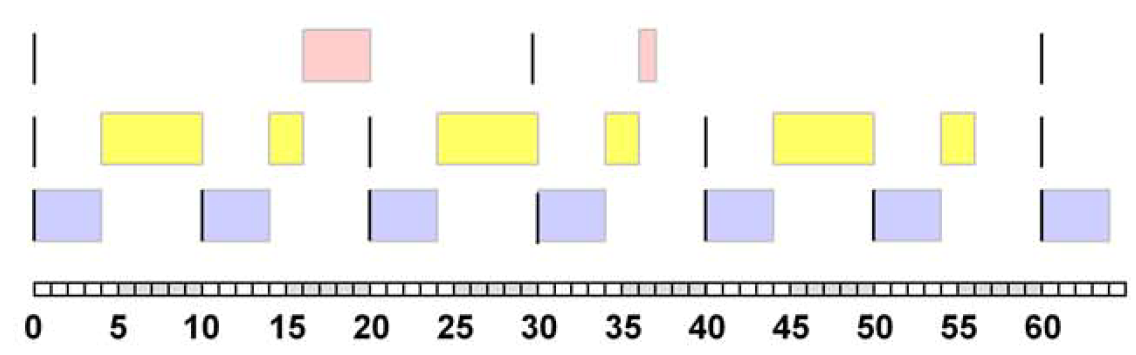
\includegraphics[scale=0.45]{./pictures/rateMonotonicSched.png}
					& \raisebox{1.25cm}{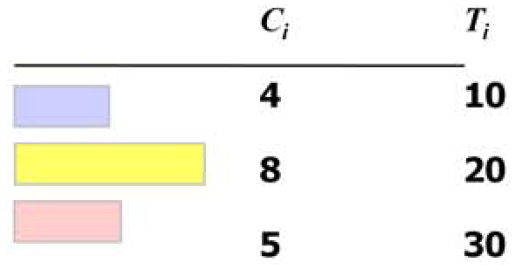
\includegraphics[scale=0.35]{./pictures/rateMonotonicCiTi.png}}\\
			\end{tabular}
		\end{table}
		
	\subsection{Voltage Scheduling}	
		Voltage Scheduling reduces the voltage of the processor (and hence the clock frequency) in order to save power. It saves energy to execute jobs as slowly as possible while still satisfying all timing constraints. \\		
	
		\begin{longtable}{p{0.4\linewidth}p{0.55\linewidth}}
			\vspace{0pt}
			
			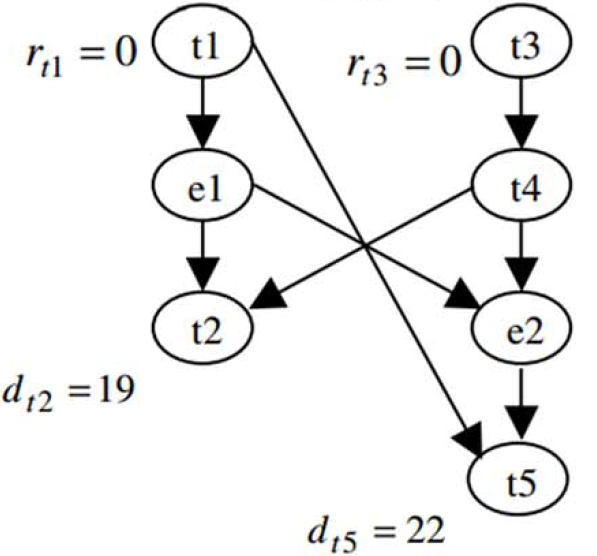
\includegraphics[scale=0.75]{./pictures/voltage_scheduling_bindings.png}
			&
				\begin{compactenum}
					\item Find the critical paths. In the above example the critical paths are:
					\begin{compactitem}
						\item Candidate 1: t1$\rightarrow$e1$\rightarrow$t2
						\item Candidate 2: t1$\rightarrow$e1$\rightarrow$e2$\rightarrow$t5
					\end{compactitem}
					The following paths are no critical paths, because in the initial schedule, they have pauses in between the tasks. 
					\begin{compactitem}
						\item Candidate 3: t3$\rightarrow$t4$\rightarrow$e2$\rightarrow$t5, pause between t4 and e2
						\item Candidate 4: t3$\rightarrow$t4$\rightarrow$t2, pause between t4 and t2
					\end{compactitem} 
				\end{compactenum}\\
			
			\vspace{0pt}
			
			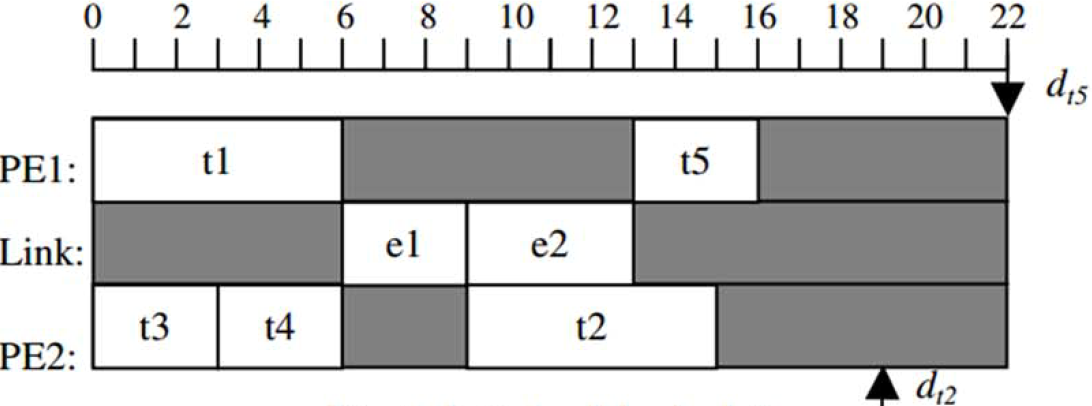
\includegraphics[scale=0.26]{./pictures/voltage_scheduling_1.png}
			
			Initial valid schedule
			& 		
				\begin{compactenum}
					\setcounter{enumi}{1}
					\item Calculate the scale for all candidates with the following formula
					\begin{equation*}
						\begin{aligned}
							scale&=\frac{D_{destination}-R_{source}}{\sum_{i}C_i} \\
							D &= \text{Deadline} \\
							R &= \text{Release time} \\
							C &= \text{Computing time}
						\end{aligned}
					\end{equation*}
					\begin{compactitem}
						\item Candidate 1: $\frac{D_{t2}-R_{t1}}{C_{t1}+C_{e1}+C_{t2}}=\frac{19-0}{6+3+6}=\frac{19}{15}$
						\item Candidate 2: $\frac{22}{16}$
					\end{compactitem}
				\end{compactenum}\\
				
			\vspace{0pt}
			
			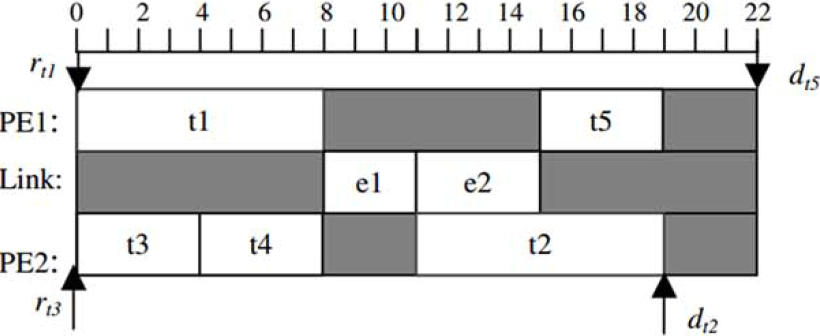
\includegraphics[scale=0.35]{./pictures/voltage_scheduling_2.png}
			
				Task execution times multiplied by a ratio of 16/12 (Step 5)			
			&
				\begin{compactenum}	
					\setcounter{enumi}{2}
					\item Select the smaller critical path $\rightarrow$ Candidate 1
					\item To fill the slack, calculate the task scaling factor with the following formula 
					\begin{equation*}
						scale=\frac{D_{destination}-R_{source}-\sum_{i}C_i}{\sum_{i\_on\_processor}C_i}+1
					\end{equation*}
					\begin{compactitem}
						\item Candidate 1: $\frac{D_{t2}-R_{t1}-(C_{t1}+C_{e1}+C_{t2})}{C_{t1}+C_{t2}}+1=\frac{19-0-15}{6+6}+1=\frac{16}{12}$
					\end{compactitem}				
				\end{compactenum}\\				
				
			\vspace{0pt}
			
			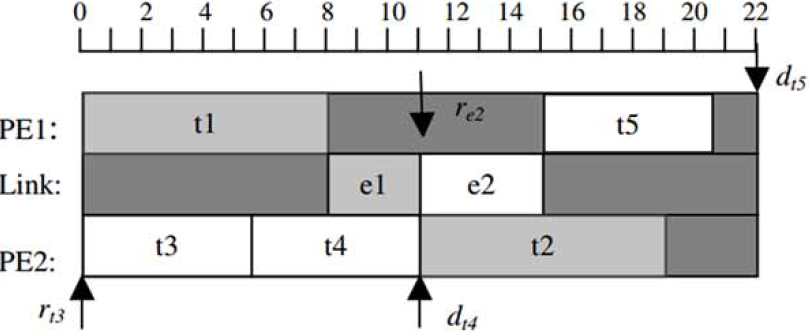
\includegraphics[scale=0.35]{./pictures/voltage_scheduling_3.png}
			
			Task execution times multiplied by a ratio of 11/8 (Step 8)			
			&
				\begin{compactenum}[\ ]
					\item As the task time of the communication task (e1) cannot be made larger or smaller the divisor consists only of the sum of the computing time of the two relevant tasks, in this case t1 and t2.
				\end{compactenum}
				\begin{compactenum}	
					\setcounter{enumi}{4}
					\item Multiply all task times (except the communication tasks (e1 and e2)) by this factor.
					\begin{compactitem}
						\item for example t1: $6*\frac{16}{12}=8$
					\end{compactitem}
					\item Remove this path from the schedule
					\item Get the next critical path. Because e1 is immovable, the next critical path is t3$\rightarrow$t4								
				\end{compactenum}	\\
			
			\vspace{0pt}
				
			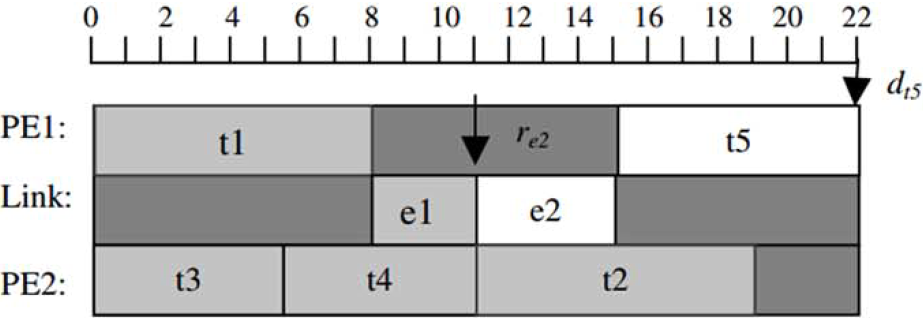
\includegraphics[scale=0.3]{./pictures/voltage_scheduling_4.png}
			
			Task execution times multiplied by a ratio of 7/5.5 (Step 11)			
			&
				\begin{compactenum}	
					\setcounter{enumi}{7}
					\item Calculate the scaling factor and scale all remaining tasks (t3, t4 and t5)
					\item Remove this path from the schedule	
					\item Get the next critical path: t5
					\item Calculate the scaling factor and scale all remaining tasks (t5)
					\item Remove this path from the schedule
				\end{compactenum}	\\
		\end{longtable}
	
%	The scaling factors for the tasks can be calculated as follows:
%	
%	\begin{equation*}
%		\begin{aligned}
%			scale_j&=\frac{d_{destination}-r_{source}}{\sum_{i}worst\_exec\_time_i} \\
%			task\_scale_j&=\frac{d_{destination}-r_{source}-\sum_{i}worst\_exe\_time_i}{\sum_{i\_on\_processor}worst\_exec\_time_i}+1 \\
%		\end{aligned}
%	\end{equation*}\\
%	& \todo{WTF does this equation even mean!?}
%	
%	
%	\\
%	Initial valid schedule & Task execution times multiplied by a ratio of 16/12 \\
%	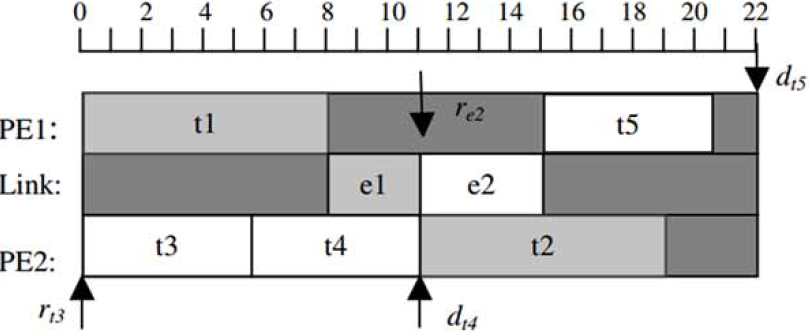
\includegraphics[scale=0.35]{./pictures/voltage_scheduling_3.png}
%	& 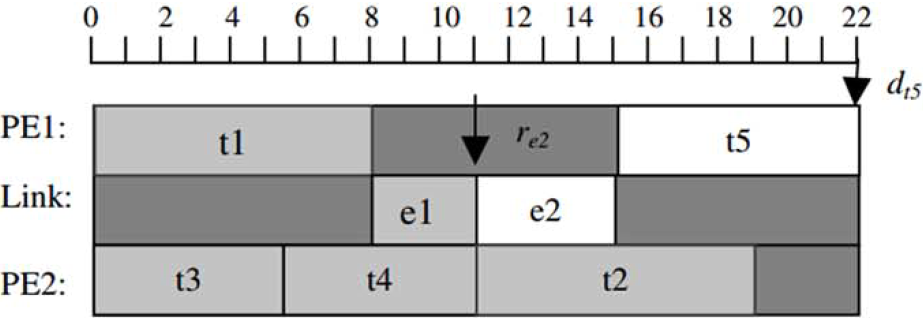
\includegraphics[scale=0.3]{./pictures/voltage_scheduling_4.png}\\
%	Task execution times multiplied by a ratio of 11/8 & Task execution times multiplied by a ratio of 7/5.5 \\